\documentclass[c]{beamer}
\usepackage[utf8]{inputenc} 
\usepackage[T1]{fontenc}
\usepackage{verbatim}
\usepackage{amsmath}
\usepackage{amsfonts}
\usepackage{amssymb}
\usepackage{lmodern}
\usepackage{graphicx}
\usepackage{enumerate}
\usepackage{stmaryrd}
\usepackage{wrapfig} 
\usepackage{tikz}

\title{Our processor}
\author{Nicolas Blanchard, Axel Davy et Marc Heinrich}
\institute{Ecole Normale Supérieure}
\date{Mardi 22 janvier 2013}
\usetheme{JuanLesPins}
\begin{document}

\begin{frame}
  \titlepage
\end{frame}

\begin{frame}
  \tableofcontents
\end{frame}

\section{Processor details}

\subsection{Inner working}
\begin{frame}
  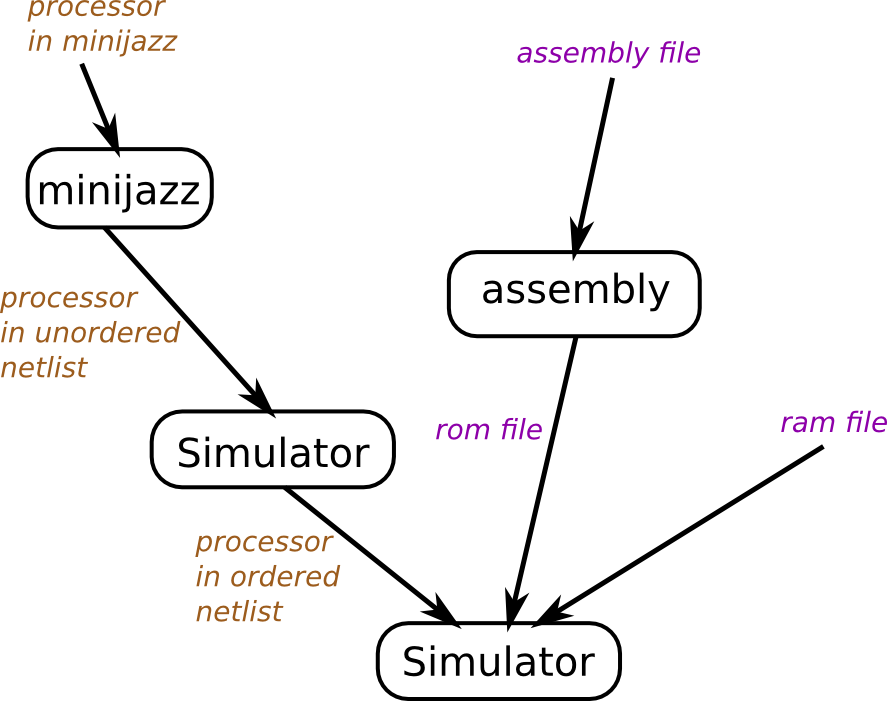
\includegraphics[scale=0.4]{schema_fonctionnement.png}
\end{frame}

\subsection{Simulator}

\begin{frame}
\begin{itemize}
\item a table for constants and variables
%\item associate to each variable appearing in the netlists equations a cell
%  in a table containing its value
\newline
\item two tables for the content of the RAM and the ROM
%\item two other tables are used to store the content of the RAM and the ROM (initialized with the files given in argument)
\newline
\item the netlist equations are applied in a specific order.
\newline
%\item outputs values, or eventually some of the cells in the RAM table are
%printed into the standard output.
\item outputs values are printed.
\newline
%\item the process goes on until it reaches the number of steps asked by the users.
\item never stops or stops after a number of steps
\end{itemize}
\end{frame}


\subsection{Assembler - rom file}

\begin{frame}
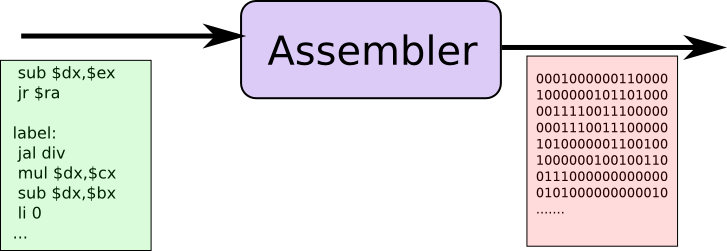
\includegraphics[scale = 0.5]{assembler.png}
%dessin au lieu de phrase
%We can put some of the architecture here
%maybe important instructions supported by our processor
%labels inplemented
%
\end{frame}

\begin{frame}
256 16 \\
0111000010000000 \\
1011000001000000 \\
0111000000000000 \\
1011000001100000 \\
0111000010000000 \\
1011000010100000 \\
0110000010001010 \\
1000000010000100 \\
0111000000111100 \\
...............
\end{frame}

\begin{frame}
\frametitle{clock program}
%maybe a picture of the assembly file (and a part of the rom file?)
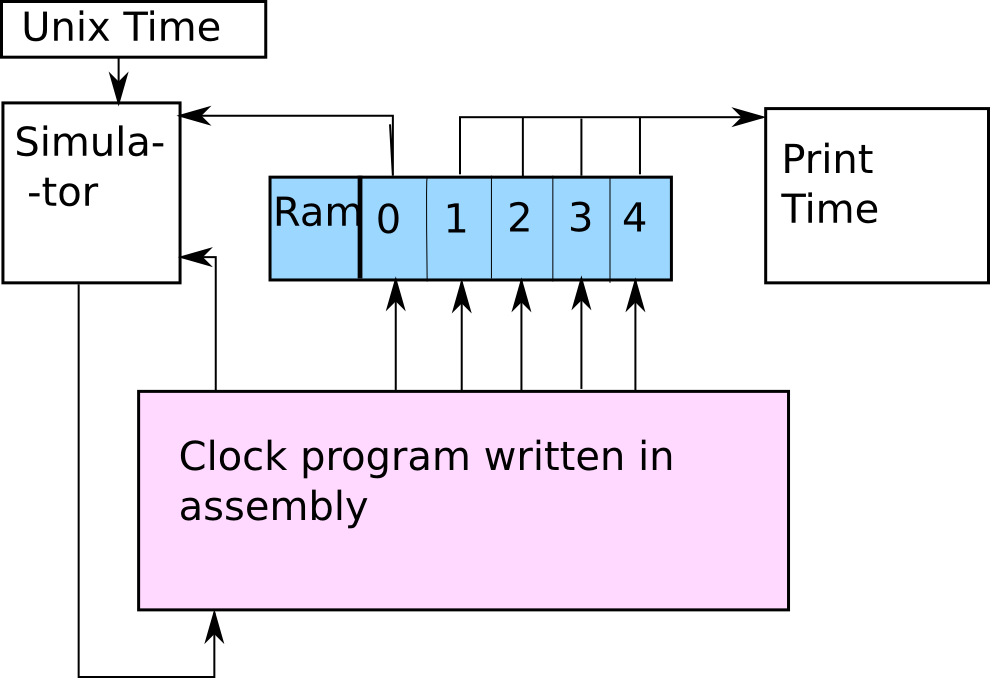
\includegraphics[scale = 0.3]{clock.png}
% copie ecran horloge en fonctionnement ou plutot schema avec cases ram
% utilises, ...
\end{frame}

\subsection{Fichier ram}

\begin{frame}
256 8 \\
0-4;  \\
00000000\\
00000000\\
00000000\\
00000000\\
00000000\\
00000000\\
00000000\\
.....
%exemple de fichier ram
\end{frame}

\subsection{Processor architecture}

\begin{frame}
\frametitle{The processor}
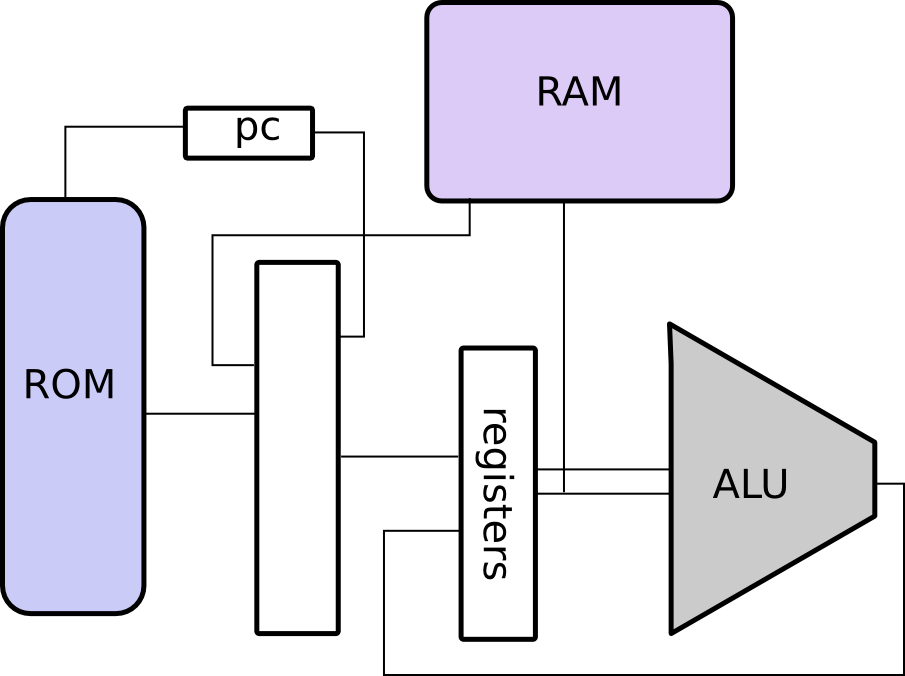
\includegraphics[scale=0.4]{schema_proc.png}

\end{frame}

\begin{frame}
\frametitle{Advantages}
\begin{itemize}
  \item Fast \pause
  \item Reliable \pause
  \item Adapted to embedded system 
  \item does not contain unuseful functions
  \item cheap
  \item energy efficient

\end{itemize}
\end{frame}

\section{Teamwork}

\begin{frame}
\frametitle{Work organization}
\begin{itemize}
\item github
\item mails
\item two ways of working
\end{itemize} 
\end{frame}

\section{Demonstration}

\begin{frame}
Demonstration
\end{frame}


\end{document}
